% Author: Joseph Rowell
% Version: 3.0
% This work is licensed under a Creative Commons Attribution 4.0 International License.
\documentclass[12pt, a4paper]{report}
\usepackage[a4paper, total={6.25in, 8.25in}]{geometry} %%%%%% CHECK MARGIN REQ. 8.25 in?
% References
\usepackage{natbib}
\setcitestyle{authoryear,open={(},close={)}}

\usepackage{multirow}
%\usepackage{multicol}
\usepackage{array}

\usepackage[T1]{fontenc}
\usepackage[utf8]{inputenc}
\usepackage[english]{babel}
\usepackage{siunitx}
\usepackage{graphicx}
\usepackage{tipa} % for the \ark{} command
\usepackage{graphics} % for pdf, bitmapped graphics files
%\usepackage{times} % assumes new font selection scheme installed
\usepackage{amsmath}
\usepackage{latexsym}
\usepackage{amscd}% for commutative diagrams
\usepackage{mathrsfs} %this package is for the script font \mathscr
\usepackage{relsize}
\usepackage{delarray}

\usepackage{graphicx} % for youtube image link

\usepackage{datatool}% Sorted list http://ctan.org/pkg/datatool

\usepackage{xcolor} % highlight text 
\usepackage[nottoc]{tocbibind} % Adds bibliography to TOC
%Also adds roman numeral pages to TOC

\usepackage{glossaries}

\usepackage{pstricks}
\usepackage{theorem}
\usepackage{changepage}
\usepackage{euscript}
\usepackage{textcomp}
\usepackage{esvect}
\usepackage{parskip}
\usepackage{placeins}
\usepackage{subfigure}
%\usepackage{subcaption}
\usepackage{array}
\usepackage{delarray}
\usepackage{stmaryrd}
\usepackage{fancyhdr}
\usepackage{graphpap}
\usepackage{makeidx}
\usepackage{enumerate}
\usepackage{esint}
\usepackage{datetime}
\usepackage{caption}
\usepackage{smartdiagram}
\usesmartdiagramlibrary{additions}
%Set Abstract Page
\usepackage{abstract}
\setlength{\absleftindent}{-5mm}
\setlength{\absrightindent}{-5mm}

%Colour definitions - put before TikZ
\usepackage{color}
\definecolor{igreen}{rgb}{0.0, 0.56, 0.0}
\usepackage{xcolor, colortbl}
\colorlet{gred}{-red!75!green!65!}
\colorlet{mamber}{-red!75!green!15!blue!50!}
\colorlet{grown}{-red!75!blue!20!green}
\colorlet{bled}{-red!85!blue!40!green!45!}
\colorlet{waters}{cyan!25} % Define color for the water
\colorlet{water}{cyan!25!green!20!} % Define color for the water
\definecolor{grin}{HTML}{00F9DE}
\usepackage{rotating}
\providecommand{\keywords}[1]{\textbf{\textit{Keywords---}} #1}

% For faint dotted table line
\usepackage{arydshln}
\setlength{\dashlinedash}{.4pt}
\setlength{\dashlinegap}{.8pt}

\usepackage{booktabs}
\usepackage{graphicx}
\usepackage{tikz}

% Added by me
\def\checkmark{\tikz\fill[scale=0.5](0,.35) -- (.25,0) -- (1,.7) -- (.25,.15) -- cycle;}

\usepackage{tikz-3dplot}
\usetikzlibrary{
arrows,
arrows.meta,
automata,
backgrounds,
calc,
decorations,
decorations.pathmorphing,
decorations.pathreplacing,
decorations.fractals,
external,
fit,
matrix,
petri,
positioning,
shadows,
shapes,
shapes.multipart,
topaths,
intersections
}
\usepackage{eso-pic}
\def\ba{\begin{array}}
\def\ea{\end{array}}
\def\beann{\begin{eqnarray*}}
\def\eeann{\end{eqnarray*}}
\def\bea{\begin{eqnarray}}
\def\eea{\end{eqnarray}}
\def\bsy{\boldsymbol}
\def\gray#1{{\color{gray}#1}}

%% COUNTERS
\setcounter{MaxMatrixCols}{20}
\renewcommand{\thesection}{\arabic{section}}
\renewcommand{\thesection}{\thechapter.\number\numexpr\value{section}}
\renewcommand{\thesubsection}{\thesection.\number\numexpr\value{subsection}}
%%For changemargin
\def\quote{\list{}{\rightmargin\leftmargin}\item[]}
\let\endquote=\endlist 
\def\changemargin#1#2{\list{}{\rightmargin#2\leftmargin#1}\item[]}
\let\endchangemargin=\endlist 
\makeatletter
\newlength\qvec@height
\newlength\qvec@depth
\newlength\qvec@width
\newcommand{\qvec}[2][]{
    \settoheight{\qvec@height}{$#2$}
    \settodepth{\qvec@depth}{$#2$}
    \settowidth{\qvec@width}{$#2$}
  \def\qvec@arg{#1}
  \raisebox{.2ex}{\raisebox{\qvec@height}{\rlap{% 
    \kern.05em
    \begin{tikzpicture}[scale=1,shorten >=-3pt,shorten <=-3pt]
    \pgfsetroundcap
    \coordinate (Stx) at (.05em,0) ;
		\coordinate (Arx) at (\qvec@width-.05em,0) ;
    \draw[->](Stx) to[bend left] (Arx);
    \end{tikzpicture}
  }}}
  #2
}
\makeatother
\makeatletter
\newlength\pvec@height
\newlength\pvec@depth
\newlength\pvec@width
\newcommand{\pvec}[2][]{
    \settoheight{\pvec@height}{$#2$}
    \settodepth{\pvec@depth}{$#2$}
    \settowidth{\pvec@width}{$#2$}
  \def\pvec@arg{#1}
  \raisebox{.2ex}{\raisebox{\pvec@height}{\rlap{% 
    \kern.05em
    \begin{tikzpicture}[scale=1,shorten >=-3pt,shorten <=-3pt]
    \pgfsetroundcap
    \coordinate (Stx) at (.05em,0) ;
		\coordinate (Arx) at (\pvec@width-.05em,0) ;
    \draw[->](Stx) to[bend right] (Arx);
    \end{tikzpicture}
  }}}
  #2
}
\makeatother
\makeatletter
\newlength\vvec@height%
\newlength\vvec@depth%
\newlength\vvec@width%
\newcommand{\vvec}[2][]{%
  \ifmmode%
    \settoheight{\vvec@height}{$#2$}%
    \settodepth{\vvec@depth}{$#2$}%
    \settowidth{\vvec@width}{$#2$}%
  \else 
    \settoheight{\vvec@height}{#2}%
    \settodepth{\vvec@depth}{#2}%
    \settowidth{\vvec@width}{#2}%
  \fi%
  \def\vvec@arg{#1}%
  \def\vvec@dd{:}%
  \def\vvec@d{.}%
  \raisebox{.2ex}{\raisebox{\vvec@height}{\rlap{%
    \kern.05em%
    \begin{tikzpicture}[scale=1]
    \pgfsetroundcap
    \draw (.05em,0)--(\vvec@width-.05em,0);
    \draw (\vvec@width-.05em,0)--(\vvec@width-.15em, .075em);
    \draw (\vvec@width-.05em,0)--(\vvec@width-.15em,-.075em);
    \ifx\vvec@arg\vvec@d%
      \fill(\vvec@width*.45,.5ex) circle (.5pt);%
    \else\ifx\vvec@arg\vvec@dd%
      \fill(\vvec@width*.30,.5ex) circle (.5pt);%
      \fill(\vvec@width*.65,.5ex) circle (.5pt);%
    \fi\fi%
    \end{tikzpicture}%
  }}}%
  #2%
}
\makeatother
\def\ba{\begin{array}}
\def\ea{\end{array}}
\def\beann{\begin{eqnarray*}}
\def\eeann{\end{eqnarray*}}
\def\bea{\begin{eqnarray}}
\def\eea{\end{eqnarray}}
\def\bsy{\boldsymbol}
\def\gray#1{{\color{gray}#1}}
\usepackage{titlesec}
\usepackage{multirow}
%To reference within text
\usepackage{hyperref}
%\usepackage{ieeetr}
\usepackage{lipsum}
\usepackage{tikz-cd}
\usepackage{float}
\usepackage{titling}
\usepackage{epigraph}
\usepackage[title, titletoc]{appendix}
\setlength\epigraphwidth{8cm}
\setlength\epigraphrule{0pt}

\titleformat{\chapter}{\normalfont\LARGE}{\thechapter\,$\vert$}{20pt}{\LARGE}{\setcounter{chapter}{0}}
\setlength{\headheight}{15pt}
\titlespacing*{\chapter}{0pt}{-70pt}{40pt} %Move chapter titles up
% Title page logos:
\makeatletter
\newcommand\BackgroundPicturea[3]{
	\setlength{\unitlength}{1pt}
	\put(0,\strip@pt\paperheight){
		\parbox[t]{\paperwidth}{
			\vspace{#2}\hspace{#3}
			\mbox{\includegraphics[scale=0.5]{#1}}
}}}
\newcommand\BackgroundPictureb[3]{
	\setlength{\unitlength}{1pt}
	\put(0,\strip@pt\paperheight){
		\parbox[t]{\paperwidth}{
			\vspace{#2}\hspace{#3}
			\mbox{\includegraphics[scale=0.3]{#1}}
}}}
\makeatother
% For my abbreviations
\newcommand{\abbrlabel}[1]{\makebox[3cm][l]{\textbf{#1}\ \dotfill}}
\newenvironment{abbreviations}{\begin{list}{}{\renewcommand{\makelabel}{\abbrlabel}}}{\end{list}}
% Line Spacing%%%%%%%%%%%%%%%%%%%%%%%%%%%%%%%%%
\usepackage{setspace}
\setstretch{1.5}
%Set of command is for the changemargin environment
\def\quote{\list{}{\rightmargin\leftmargin}\item[]}
\let\endquote=\endlist 
\def\changemargin#1#2{\list{}{\rightmargin#2\leftmargin#1}\item[]}
\let\endchangemargin=\endlist
%Replace Contents to Table of Contents	
\addto\captionsenglish{
	\renewcommand{\contentsname}%
	{Table of Contents}
	\setcounter{tocdepth}{3}% Include \subsubsection in ToC
	\setcounter{secnumdepth}{3}% Number \subsubsection in ToC
	}
\renewcommand{\listfigurename}{List of Figures}
\renewcommand{\listtablename}{List of Tables}


\usepackage{xcolor}
\usepackage{listings}
\usepackage{xcolor}

%New colors defined below
\definecolor{codegreen}{rgb}{0,0.6,0}
\definecolor{codegray}{rgb}{0.5,0.5,0.5}
\definecolor{codepurple}{rgb}{0.58,0,0.82}
\definecolor{backcolour}{rgb}{0.95,0.95,0.92}

%Code listing style named "mystyle"
\lstdefinestyle{mystyle}{
  backgroundcolor=\color{backcolour}, commentstyle=\color{codegreen},
  keywordstyle=\color{magenta},
  numberstyle=\tiny\color{codegray},
  stringstyle=\color{codepurple},
  basicstyle=\ttfamily\footnotesize,
  breakatwhitespace=false,         
  breaklines=true,                 
  captionpos=b,                    
  keepspaces=true,                 
  numbers=left,                    
  numbersep=5pt,                  
  showspaces=false,                
  showstringspaces=false,
  showtabs=false,                  
  tabsize=2
}

%"mystyle" code listing set
\lstset{style=mystyle}
\lstset{basicstyle=\tiny,style=mystyle} 

\renewcommand\lstlistingname{Listing}
\renewcommand\lstlistlistingname{Listings}
\def\lstlistingautorefname{Alg.}

\usepackage{amsfonts}
\newcommand{\R}{\mathbb{R}}
\newcommand{\U}{\mathbb{U}}
\newcommand{\I}{\mathbb{I}}

%% Sorted list
\newcommand{\sortitem}[1]{%
  \DTLnewrow{list}% Create a new entry
  \DTLnewdbentry{list}{description}{#1}% Add entry as description
}
\newenvironment{sortedlist}{%
  \DTLifdbexists{list}{\DTLcleardb{list}}{\DTLnewdb{list}}% Create new/discard old list
}{%
  \DTLsort{description}{list}% Sort list
  \begin{itemize}%
    \DTLforeach*{list}{\theDesc=description}{%
      \item[] \theDesc}% Print each item, remove [] for bullet
  \end{itemize}%
}
%% 

% Algorithms and pseudocode packages
\usepackage{algorithm}
\usepackage{algpseudocode}


%Gantt chart
\usepackage{pgfgantt}

\usepackage{makecell} %multiline in tables

\usepackage{lscape}


\usepackage{multicol}
\hypersetup{pdftitle = Project Report, pdfauthor = {First Last}, pdfstartview=FitH, pdfkeywords = essay, pdfpagemode = FullScreen, colorlinks, anchorcolor = black, citecolor = black, urlcolor = blue, filecolor = green, linkcolor = black, plainpages = false}
%%%%%%%%%%%%%%%%%%%%%%%%%%%%%%%%%%%%%%%%%%%%%%%%%%%%%%%%%%%%%%%%%%%%%%%
%\pagestyle{fancy}
\rhead{}
\chead{}
\lhead{University College London}
\lfoot{\date{}}
\cfoot{}
\rfoot{\thepage}
% Top and Bottom Line Rules

\renewcommand{\headrulewidth}{0.4pt} %0.4pt
\renewcommand{\footrulewidth}{0.4pt}
\fancyheadoffset{8pt}
\fancyfootoffset{8pt}
% Line spacing
\renewcommand{\baselinestretch}{1.5} %1.5

\makeglossaries

\newglossaryentry{latex}
{
    name=Latex,
    text=latex,
    description={Is a markup language specially suited 
    for scientific documents, this term is printed in conclusion }
}
\newglossaryentry{raster}
{
    name=Raster,
    text=raster,
    description={ images are compiled using pixels, or tiny dots, containing unique color and tonal information that come together to create the image }
}
\newglossaryentry{gradient descent}
{
    name=Gradient descent,
    text=gradient descent,
    description={Is a naive optimization method which consists of steepest descent down the gradient of the given cost function}
}

\newglossaryentry{Gauss-Newton}
{
    name=Gauss-Newton,
    description={Is a Newton-like method for solving a non-linear least squares problem, in which the Hessian $H$ is approximated by $H \approx J^T WJ$, where $J$ is the design matrix and $W$ is the weights. The normal equations are the resulting prediction equations given as \\ $(J^TWJ) \delta x = -(JW \Delta z)$}
}

\newglossaryentry{Conjugate Gradient}
{
    name=Conjugate Gradient,
    text=conjugate gradient,
    description={Is an accelerated first order iterative process for solving positive definite linear systems or minimizing a non linear cost function.}
}

\newglossaryentry{Jacobian}
{
    name=Jacobian,
    description={Matrix of partial differentials of the cost function $J = \frac{df}{dx}$}
}

\newglossaryentry{Hessian}
{
    name=Hessian,
    description={Matrix of second partial differentials of the cost function $H = \frac{d^2f}{dx^2}$}
}
\newglossaryentry{Gradient}
{
    name=Gradient,
    description={First differential $g = \frac{df}{dx}$}
}
\newglossaryentry{epipolar plane}
{
    name=Epipolar Plane,
    description={The plane containing the intersection line joining the camera centres with the image plane.}
}
\newglossaryentry{linear least squares}
{ 
    name =Linear Least Squares,
    description ={Least squares approximation of linear functions to data, by minimizing residuals.
     $E_{LS} = \sum_i{||\hat{x'_i}- \tilde{x'_i}||}$}
}
\newglossaryentry{RANdom Sample Consensus (RANSAC)}
{
    name = Random Sample Consensus (RANSAC),
    description = {An iterative method to estimate parameters of a mathematical model from a set of observed data which contains outliers.}
}


\date{August 2023}

\title{Accessibility impact of transport infrastructure: Spatial assessment of Bogot\'{a}\textquotesingle s future metro system}
\author{\\ \Large{Andr\'{e}s Restrepo Jim\'{e}nez}
\\ Supervisor: Dr. Fulvio Lopane 
\\ Module: CASA0010
%\\ The Bartlett Faculty of the Built Environment
%\\ Centre for Advanced Spatial Analysis
\\
\\ Remote repo link
\\ Word count: XXXXX
\\
%\\ University College London
\\
This dissertation is submitted in part requirement for \\the \textit{MSc Urban Spatial Science} in the \\Centre for Advanced Spatial Analysis, \\Bartlett Faculty of The Build Environment, \\University College London.
\\ \\
% \\Disclaimer:This report is submitted as part requirement for the MSc in Robotics  and Computation at University College London. It is substantially the result of my own work except where explicitly indicated in the text.The report may be freely copied and distributed provided the source is explicitly acknowledged.
% September 2022
}
%\hypersetup{citecolor=black}
%%%%%%%%%%%%%%%%%%%%%%%%%%%%%%%%%%%%%%%%%%%%%%%%%%%%%%%%%%%%%%%%%%%%%%%
\begin{document}
%Adjust logo positions here
% \AddToShipoutPicture*{\parbox[t][\paperheight][t]{\paperwidth}{%
%           \includegraphics[width=\paperwidth]{\BackgroundPicturea{Logos/ucl_long%_logo.png}{3in}{3in}}
%           }}
% \AddToShipoutPicture*{\centering\BackgroundPictureb{Logos/Bentham2011_065_c623d.jpg}{3in}{3.7in}}
\AddToShipoutPictureBG*{%
  \AtPageUpperLeft{%
    \raisebox{-\height}{%
      
\includegraphics[width=\paperwidth]{Logos/UCL page header_V1.png}%
    }}
}
\AddToShipoutPicture*{%
      \parbox[t][\paperheight][t]{\paperwidth}{%
          
\includegraphics[width=1.2\paperwidth]{Logos/UCL page footer.png}
      }}
      

\thispagestyle{headings}
\maketitle
\FloatBarrier
\pagenumbering{roman}

\thispagestyle{empty}
\begin{abstract}
%\lipsum[5]
Testing absttact
%1.Talks about general application or general field of research
%2. Explains the challenge that is not answered yet
%3. Describe idea for tackling that challenge e.g. overall idea
%4 Methodology undertaken in research  e.g. tools, methods, steps taken.
%5. Main achievement of research supported by numerical results
%6. comparison with similar research in literature (qualitatively or quantitatively), and/or explain possible future applications of outcomes


\keywords{keyword 1 - keyword 2 - keyword 3}
% \vspace{-10mm} %To remove added white space after
\end{abstract}
\newpage
\thispagestyle{empty}
\begin{center}
I dedicate this ...
\end{center}

\newpage
\thispagestyle{empty}
\vspace*{\fill}
\begin{center}
Copyright \copyright  \thinspace 2023 by Andr\'{e}s Restrepo Jim\'{e}nez \\ All Rights Reserved
\end{center}
\vspace*{\fill}
\newpage
\thispagestyle{empty}
%\epigraph{The Book of Nature is written in the language of mathematics.}{--- \textup{Galileo Galilei}}
\epigraph{The computer was born to solve problems that did not exist before.}{--- \textup{Bill Gates}}


\thispagestyle{empty}
\chapter*{Acknowledgements}


\thispagestyle{empty}
\chapter*{Declaration}
I, Andr\'{e}s Restrepo Jim\'{e}nez, hereby declare that this dissertation is all my own original work and that all sources have been acknowledged. It is xxx words in length. \\
Add signature png here.
\begin{figure}[H]

\includegraphics{Logos/Signature.jpg}
\end{figure}
\vspace{-2cm}
\noindent\begin{tabular}{ll}
 & 20/08/23 \\
\makebox[2.5in]{\hrulefill} & \makebox[2.5in]{\hrulefill}\\
\textit{Signature} & \textit{Date}\\
\end{tabular}


\tableofcontents
\pagenumbering{arabic}
\thispagestyle{plain}
\listoffigures
\listoftables
%\lstlistoflistings
%\listofalgorithms


%\begin{singlespace}
\chapter*{List of acronyms or abbreviations}
\begin{sortedlist} %sort alphabetically
  \sortitem{BRT: Bus rapid transit}
  \sortitem{GIS: Geopraphic information system}
  \sortitem{GTFS: General transit feed specification}
  \sortitem{GDP: Gross domestic product}
  \sortitem{SDP: Sustainability development goal}
  \end{sortedlist}
% \end{singlespace}
%%%%%%%%%%%%%%%%%%%%%%%%%%%%%%%%%%%%%%%%%%%%%%%%%%%%%%%%%%%%%%%%%%%%%%%%%%%%%%%%
%\input{1 Introduction}
%%%%%%%%%%%%%%%%%%%%%%%%%%%%%%%%%%%%%%%%%%%%%%%%%%%%%%%%%%%%%%%%%%%%%%%%%%%%%%%%
%\input{2 Literature review}
%%%%%%%%%%%%%%%%%%%%%%%%%%%%%%%%%%%%%%%%%%%%%%%%%%%%%%%%%%%%%%%%%%%%%%%%%%%%%%%%
%\input{3 Study area and or data chapter}
%%%%%%%%%%%%%%%%%%%%%%%%%%%%%%%%%%%%%%%%%%%%%%%%%%%%%%%%%%%%%%%%%%%%%%%%%%%%%%%%
%\input{4 Methodology}
%%%%%%%%%%%%%%%%%%%%%%%%%%%%%%%%%%%%%%%%%%%%%%%%%%%%%%%%%%%%%%%%%%%%%%%%%%%%%%%%
%\input{5 Results}
%%%%%%%%%%%%%%%%%%%%%%%%%%%%%%%%%%%%%%%%%%%%%%%%%%%%%%%%%%%%%%%%%%%%%%%%%%%%%%%%
%\input{6 Discussion}
%%%%%%%%%%%%%%%%%%%%%%%%%%%%%%%%%%%%%%%%%%%%%%%%%%%%%%%%%%%%%%%%%%%%%%%%%%%%%%%%
%\input{7 Conclusion}
%%%%%%%%%%%%%%%%%%%%%%%%%%%%%%%%%%%%%%%%%%%%%%%%%%%%%%%%%%%%%%%%%%%%%%%%%%%%%%%%

\chapter{Introduction} \label{Chap1}

\section{Background}

% The first announcement of the construction of Bogota's future metro system was on XXXXXX by XXXX. 

On several occasions, the need for a higher-capacity public transportation system in Colombia's capital has taken great attention from the general public. The initial idea of building a metro in Bogot\'{a} goes back to the year 1942 when the current mayor at the time suggested the building of a new metro system as the functioning trolley car was highly demanded \citep{metrodebogotaHistoriaMetroBogota2011}. The previous versions of the project were unsuccessful in terms of their execution and compilation, however, each attempt reinforced the need of improving Bogota's public transportation system.

The scale and dimension of Colombia's capital, Bogot\'{a} can be measured from multiple angles. Population-wise, with 7.9 million people, it is the country's biggest city and accounts for 15\% of the country's total population, as Medell\'{i}n and Cali take second and third place with 5\% and 4\% of the total population, respectively \citep{daneProyeccionesPoblacionPopulation2023}. Regarding the city's economic role, it is the biggest economic hub with 25\% of the nation's GDP, followed similarly as in the population distribution by Medell\'{i}n and Cali, with 6\% and 4\%, respectively \citep{daneCuentasNacionalesDepartamentales2023}.

Currently, the main mode of transportation in the city is a bus rapid transit (BRT) system that accounts for approximately 36\% of the total daily trips \citep{alcaldiadebogotad.c.EncuestaMovilidad20192019}. Given the rapid population growth in Colombia's capital during the last decades of the 20th century, the 'Transmilenio' system started operations in the early '00s and was intended to provide a cost-efficient transport solution \citep{rodriguezValueAccessibilityBogota2004}. 

By September 2016, the local and national governments finally materialized their intentions in a formal agreement to support the development of the metro project which led to the ongoing construction process that started in 2021. The project consists of the construction of the first of two future metro lines. The scope of this research will only include the first metro line in the future scenario as the final designs of the second metro line have not been published yet. 

The first metro line will have a 23,9-kilometre length overground track with 16 stations. With an investment of 12,95 billion COP (4,33\footnote{September 2017 average COP/USD rate: 2.991,42 \citep{bancodelarepublicaTasaCambioRepresentativa2023}} billion USD), the construction of the first line began in 2021 and is supposed to be finished by 2028.


% \begin{itemize}
%  \item Lack of functioning metro system in Bogota although it has been proposed and mention in previous local and/or national government plans
% \end{itemize}

\section{Importance}

The improvement of the current transport infrastructure system in Colombia's capitals aims to impact a significant share of Bogot\'{a}'s population, as 1 in every 3 trips in the city relies on public transportation. According to Bogot\'{a} City Council, BRT is the primary mode of commuting, with 4,8 million trips a day \citep{EncuestaMovilidad20192019}. From the total of 13.4 million daily trips, BRT accounts for 36\% total trips, followed by walking\footnote{Pedestrian trips with length greater or equal to 15 minutes} and privately owned cars, with 24\% and 15\% of total trips, respectively.



\begin{itemize}

\item Congested BRT Network

\item Brief intro to Bogota as a city and centre of economic and decision-making processes
\item How does it contribute or prevent people to have better life quality
\item It takes advantage of the use of publicly available data from transport and local authorities (spatial and non-spatial)
  \item Provide technical tools to assess transport planning decision
  \item Baseline reference for future or similar transport public policy decision making
  \item Assess how the metro system designs address the accessibility of the inhabitants
  \item Spatial reference for future local government intervention and investment decisions from the private sector
  \item Highlight accessibility importance in an economic and urban context and How can it drive growth
  \item Mention the impact on making cities more "liveable" and contribute to having a better life quality
\end{itemize}

\section{Research question}

The present research aims to address:

% Initial one


% \begin{center}
%     \textit{How would the public transportation accessibility spatially vary with the construction of Bogot\'{a}\textquotesingle s future metro system?}
% \end{center}

% Adjusted one

% \begin{center}
%     \textit{How would Bogot\'{a}\textquotesingle s future metro lines contribute to improving access to opportunities? To what extent is addressing the socio-spatial inequalities in Colombia\textquotesingle s capital?}
% \end{center}

% Current one

\begin{center}
    \textit{How would Bogot\'{a}\textquotesingle s future metro lines contribute to improving access to opportunities? How would the public transportation accessibility spatially vary with the construction of Bogot\'{a}\textquotesingle s future metro system?}
\end{center}



% \subsection{Subsection}
% \subsubsection{SubSubsection}
% \paragraph{Parragraph}
% \lipsum[5]
% Testing \Gls{raster}

Testing footnote\footnote{Capion of footnote!}


\chapter{Literature review} \label{Chap2}

\section{Modelling in the urban context}

The use of modelling tools in the urban environment has gained popularity for analyzing high-complexity topics to support the decision-making process \citep{houApproachBuildingOccupancy2020}. As urban theories can be represented in mathematical models, the use of simulation processes allows researchers to experiment with possible outcomes in future urban scenarios \citep{battyUrbanModeling2009a}.

Regarding the urban modelling process as a discipline both, \cite{battyUrbanModeling2009a} and \cite{wilsonFutureUrbanModelling2018}, presented past references to grasp a general notion of its historic evolution. On one hand, \cite{battyUrbanModeling2009a} stated how the first formal contributions on the topic go back to \cite{alonsoLocationLandUse1964}, the basis of the so-called new urban economics. Batty included a model-building process overview listing the main scientific and mathematics principles to consider. On the other hand, \cite{wilsonScienceCitiesRegions2012} highlighted the influence of \cite{lowryModelMetropolis1964} as a milestone in the urban modelling evolution and uses it as an example to explain urban modelling together with a full historical review of the field.

Taking \cite{battyUrbanModeling2009a} and \cite{wilsonFutureUrbanModelling2018} as references, the urban models can be grouped into three main categories: 

\begin{enumerate}
  \item Land-use transportation: Conceptually based on the gravitational model \citep{battyUrbanModellingAlgorithms1976}, it aims to predict the spatial interaction (flows) between land use, economic activity and the inherent transportation costs of spatial units within the area of study. Leveraging on the principles of Newton's model, these models forecast how spatial units would  interact with one another considering the cost of interaction and attractiveness between them.
  \item Urban dynamics: Built on the principles used in ecological dynamic models and system dynamics, the urban dynamics models intend to derive the aggregate future dynamic activity or state that may result within an urban system through time.
  \item Cellular automata and agent-based modelling: They aim to simulate the emergent aggregate result of individual agent-level actions in a system, as agents interact with both the environment and other agents.
  \item Network analysis: It allows to study of the connections patterns that may arise between components to systematically assess the collective behaviour of components as a whole \citep{newmanNetworksIntroduction2010}.
\end{enumerate}

With the emergence of computational modelling, \cite{battyUrbanModeling2009a} described how it allowed urban theories to be deployed in an experimental digital environment. As theoretical knowledge can be represented in mathematical models, the use of simulation processes allowed researchers to experiment with hypothetical circumstances and produce possible outcomes in future urban scenarios \citep{battyUrbanModeling2009a}.

% Refernce to the futuro portraid by Wilson

In a more prospective and industry-related exercise, \cite{wilsonFutureUrbanModelling2018} presented his view on how urban modelling will develop and prosper in the future. Regarding tools and the inputs to further urban modelling development, \cite{wilsonFutureUrbanModelling2018} mentioned how big data and technological advancements will enable new capacities and new input data to apply modelling in the urban context. Apart from the already relatively well-developed urban modelling tools designed for transport assessment and retail location intelligence, \cite{wilsonFutureUrbanModelling2018} listed other industries that could expand spatial modelling to support their location decision-making processes. Among the high-use modelling potential situations, \cite{wilsonFutureUrbanModelling2018} mentioned the energy sector, global trading models and the defence and security industry.

% Move to other section
% Technological information developments for the last decades have enabled greater capture, storing and processing capacities \citep{krainesIntegratingDistributedComputational2011}, a more multidisciplinary and robust approach is now available when addressing built environment-related phenomena. 

Given these points, it was highlighted by \cite{battyUrbanModeling2009a} and \cite{wilsonFutureUrbanModelling2018} how these modelling tools hold great value for both policymakers and private parties, as they manage to integrate theoretical constructs or business strategies and put them to the test through computational modelling \citep{battyUrbanModeling2009a}. Either from a public, private or research perspective, modelling tools applied to the urban context could provide decision-makers with new innovative insights and possible solutions to the numerous challenges that cities and society currently face across the globe.

Furthermore, \cite{battyUrbanModeling2009a} clarified that apart from the computational models above mentioned, GIS-based models are also part of the urban modelling domain and will be described in the next section of the present document.

% Mention to the groups described by Batty, complemented with the ones described by Clarke's article




% which included the main model types, their applications and future uses for urban policy-making. 



% In order to deploy these state-of-the-art computational tools on the subject of interest, data is required. Apart from the underlying theory of the model, data that intends to capture the topic of interest is essential to leverage computational models to contribute to urban-related topics. The expansion of urban modelling is highly related to the data availability to use as input in the simulation process. Luckily, there have been enormous 

% Without input data for the modelling process, the future of urban modelling would be highly compromised, luckily that is not the case. 

% Open data

% Open government

% Data science

\section{Geographic information systems}

Geographic information can be defined as the result of combining non-spatial data with their location in space. \cite{longleyGeographicInformationScience2015} defined geographic information as data that represents the 'what' and the 'where' features of anything. The 'what' component of the data would account for the attributes or non-spatial data captured and the 'when' is responsible for holding the coordinates that symbolise a specific location on earth.

According to \cite{maclachlanAppliedGeographicInformation2022} geographic information can be divided into two main data types:

\begin{enumerate}
  \item Vector: Geographic vector data typically includes points, lines, polygons and grids.
  \item Raster: The raster format consists of a set of cell grids in which each cell holds a specific value. 
\end{enumerate}

To illustrate the use of geographic data, figure \ref{fig:Fig_data_types} shows the fashion in which data type can deliver a fair representation of the real world, through the use of both vector and raster data.

\begin{figure}[htp]
    \centering
    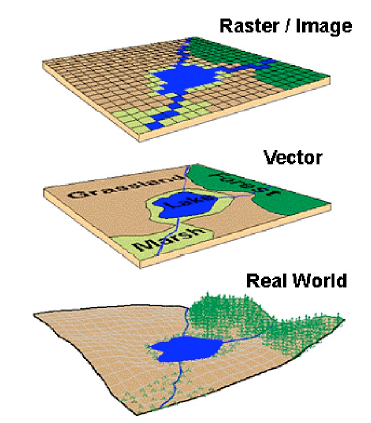
\includegraphics[width=6cm]{Images/Fig_Types_Geodata.png}
    \caption{Vector and raster geographical representation \citep{saabConceptualizingSpaceMapping2003}}
    \label{fig:Fig_data_types}
\end{figure}


% Include image of types of data: Look in \cite{longleyGeographicInformationScience2015} or use image from Andys book

The main use of geographic information is to represent the relative locations of features through a schematic and visual geographic model. With a certain level of abstraction, detail and scale, geographic modelling (mapping) produces knowledge related to the location and the features of the subject of study \citep{longleyGeographicInformationScience2015}. Hence, a geographic information system (GIS), consists of the systematic collection of geo-referenced attribute data. Gifted with powerful processing capabilities, 'GI systems are computer-based tools for collecting, storing, processing, analyzing, and visualizing geographic information' \citep{longleyGeographicInformationScience2015}.

% Geographic model

% enables one to record and represent the location  

% Abstraction and scientific method reference

% Map as a model to represent reality

% Reference to urban modelling for transport

As computing does in most cases, computer-based GIS offers the capacity of processing data in a fraction of the time that would take if is performed manually. Similarly, the generation and capture capacity of location-related attributes has widespread \citep{longleyGeographicInformationScience2015}, as the use of digital means has expanded to support all kinds of services and activities. The conjunctions of these two circumstances are aligned with the future scenario portrayed by \cite{wilsonFutureUrbanModelling2018} with the use of urban modelling covering new unattended spatial modelling and analysis needs.

When leveraging GIS technology to contribute to a specific topic or situation, the use cases vary enormously. As an example of the versatility of GIS to address location-related topics, \citep{longleyGeographicInformationScience2015} listed possible scenarios which include:

\begin{itemize}
\item Impact assessment of possible transport infrastructure.
\item Shipping route planning optimization.
\item Health services coverage.
\item Location intelligence for retailers shore expansion.
\item National parks and natural resources management.
\item Agriculture resources consumption.
\item National defence resources allocation.
\item Tourism navigation and reviewing tools.
\end{itemize}

The geo-processing involved in GIS modelling relies on a wide range of geometrical and mathematical operations. Depending on the type, nature and purpose of the modelling process, different computational procedures are performed to transform the inputs into the intended outcomes that hopefully contribute to the area of study. These methods are usually supported by processing algorithms composed of sequential simpler operations like time, distance, length and area computing. 

% As the GIS derive its operation in  geoprocessing workflows, next some examples of the intermediate results are listed:


% \begin{itemize}
% \item Geometric relations related operations.
% \item Aggregation or dis-aggregation across spatial units.
% \item Spatial and non-spatial data interrelation.
% \item Spatial subsetting.
% \item Proximity analysis.
% \item Time travel matrix computation.
% \end{itemize}

% \begin{itemize}
% \item Point pattern analysis.
% \item Spatial correlation analysis.
% \end{itemize}


In that sense, GIS can be used to address a wide range of location-sensitive topics as they enable and support spatial modelling processes to test future scenarios according to the applicable use case.

PENDING


% Illustrate intermediate results

% Feature management engineering
% Geometry operations
% Geoprocessing
% format conversion
% projection
% Aggregation


% REfenrece to specific GIS measures

\section{Accessibility modelling}

The concept of urban accessibility can be defined as the 'with which people can reach places and opportunities – or, conversely, a characteristic of places and opportunities in terms of how easily they can be reached by the population', \cite{geursAccessibilityEvaluationLanduse2004b} and \cite{neutensEquityUrbanService2010} cited by \cite{pereiraIntroductionUrbanAccessibility2023a}. Alternatively, \cite{paezMeasuringAccessibilityPositive2012} further expands the definition by framing accessibility into two main components: 'the cost of travel...and the quality/quantity of opportunities'. The cost of travel can be understood as either the monetary cost or the duration or time of the trip to reach the destination, depending on the modelling setup and purpose.

Important to realize that the universal meaning of the word accessibility can represent different concepts. \cite{pereiraIntroductionUrbanAccessibility2023a} presented how accessibility can be understood differently depending on the scale and the context where is applied. On one hand, macro or urban accessibility refers to the effortless ability of people in reaching locations of interest. On the other hand, micro-accessibility is related to how spaces are suitable for people with different levels of mobility or reasoning challenges. 


% Mobility vs accessibility

Likewise, accessibility and mobility are both terms constantly used in the transport assessment context that represent different concepts. Their main distinctive feature can be summarized 
as 'Accessibility,..., refers to the potential ability to reach activities and opportunities. While a mobility analysis would focus, for example, on the time people spend commuting...' \cite{pereiraIntroductionUrbanAccessibility2023a}. Regarding the benefits of introducing the use of accessibility measures in transport planning, \cite{ferreiraAccessibilityGoldMobility2012} argued that planning practitioners should include accessibility measures as it better captures the real benefits in transport-related assessment.

% Reference to other authors in Colombian or non-Colombian cases

From a global perspective, the aggregate results that urban accessibility provides can also be used to measure contributions related to sustainability. As the measure encapsulates the interaction between transport and opportunities, it explicitly relates to sustainability development goal \# 11 'Make cities and human settlements inclusive, safe, resilient and sustainable' \citep{unitednations17GOALSSustainable2015}. Under this sustainability development goal (SDG), both topics 'Sustainable transport' and 'Sustainable cities and human settlements' are aligned with the use of accessibility measurements, considering that it quantitatively captures the principles that these topics promote.

Regarding the interpretation and use of an accessibility-based measure, there are references in the urban development field.  

\cite{pereiraIntroductionUrbanAccessibility2023a} highlighted how it manages to holistically capture the overall result of the transportation offer, the distribution of strategically important activities and the location of individuals within the study area. Additionally, \cite{pereiraIntroductionUrbanAccessibility2023a} stated how accessibility is also related to social inclusion as it accounts for not only the current functioning transport system but also how this system allows individuals to access the location of their interest.

\cite{papaAccessibilityInstrumentsPlanning2016} and \cite{boisjolyHowGetThere2017} cited by \cite{pereiraIntroductionUrbanAccessibility2023a} stated how accessibility measures are used in transport assessment contexts. \cite{boisjolyHowGetThere2017} presented how accessibility measures favour a more systematic assessment of transportation needs being covered, although their use has not been widespread among transport planning practitioners as the authors expected. \cite{boisjolyHowGetThere2017} considered transport plans from cities in Europe, North America, Australia and Asia.
In contrast, \cite{papaAccessibilityInstrumentsPlanning2016} showcased several European examples where accessibility measures were included in the assessment considered in routine planning practices.

% Brief explanation of accessibility measures

Within accessibility, multiple measures are available to model how easily people can reach their destinations of interest. \cite{paezMeasuringAccessibilityPositive2012} and \cite{dijstOpportunitiesTransportMode2002} cited by \cite{pereiraIntroductionUrbanAccessibility2023a}, presented a general review of the main groups of accessibility measures, which are summarized and listed next:

\begin{itemize}
  \item Place-based measures: The place-based measures aim to quantity the ability to reach opportunities from a specific location in space due to the spatial distribution of opportunities and the transport network available. These measures can be grouped as follows:
    \begin{itemize}
        \item Cumulative opportunity measures: The cumulative measure considers the total of opportunities that can be reached from a given location that complies with a time or travel cost threshold.
            \begin{itemize}
                \item Active cumulative accessibility measure: It consists of the number of opportunities that a person located in a given location can access with ease within a threshold. 
                \item Passive cumulative accessibility measure: It reflects the number of people that can reach a certain destination or opportunity without exceeding the travel cost threshold.
            \end{itemize}
        \item Minimum travel cost: It maps the nearest locations of interest (opportunity) by considering the one destination with the lowest travel cost, either time or monetary cost.
        \item Gravity measures: Based on Newton's gravitational model, it accounts for variation in travel cost as the distance between the origin and destination location increases.
        \item Floating catchment area competition: The catchment area measure aims to account for the interaction between the offer of opportunities and the demand of individuals according to their spatial distribution and accessibility levels.
        
    \end{itemize}
  \item Person-based measures: In conjunction with the transport network and spatial opportunity distribution, this measure also considers the personal features of individuals in a given location in space.
\end{itemize}

% References to research



% \begin{itemize}
%   \item Success cases of the use of accessibility measures
%   \item Reference to initiatives and efforts from NGO organizations related to urban accessibility: IBD, World Bank, GIZ.
%   \item Reference to north and global south previous research
% \end{itemize}

\section{Colombia and the Bogot\'{a} study case}

In the urban development field, there is an extended list of references related to the use of accessibility applied to transport assessments context. Particular interest in research activities has been expended on areas that have experienced migration and/or relatively more rapid urbanisation processes \citep{kojimaIntroductionPopulationMigration1996}. Latin america and Colombia are not excluded from this trend as the rapid urbanization reinforces the already present inequalities in cities \citep{wrightwendelAccessibilityUsabilityGreen2012,tellezUrbanDevelopmentBogota2018}.


Colombia's capital, Bogot\'{a} has been an area of study of multiple transport and accessibility-related research exercises. That should not come as a surprise considering the population growth that Bogot\'{a} and her surrounding municipalities have experienced over the last couple of decades. By 2017, Bogot\'{a} had almost doubled its population during the last 30 years and similarly did the near municipalities by increasing their population by almost 3 times during the same time period \citep{guzmanCityProfileBogota2017}.

A milestone in Bogotá's transportation history was the operation start of its current BRT 'Transmilenio' system by the beginning of the 21st century \citep{rodriguezValueAccessibilityBogota2004}. Derived from the deployment and the integration of collective bus services in Bogotá, the resulting accessibility effect of the BRT system has been a popular element of study among transport and development-related researchers. The next paragraph intends to list the previous research exercises that have expanded on the topic of interest of the present research, however, there are clearly other valuable contributions that could not be included due to practical limitations.

% It is clear that the BRT system provided the city with a functioning solution to integrate most of the collective bus services.

Although it was not a proper accessibility assessment as defined in previous sections, \cite{rodriguezValueAccessibilityBogota2004} initially examined the relationship between proximity and land value and found that apparently there was a positive relation between the land price and the proximity to the BRT system stations. However, the influence might be underscored by the short time frame (2 years) between the measure and the operation kick-off of the BRT system.

With a more straightforward social-inequality and accessibility approach, \cite{bocarejos.TransportAccessibilitySocial2012} performed an urban accessibility assessment on the city's BRT system. Considering that their main research goal was to generate an 'analysis tool that helps quantify and differentiate access inequalities' \cite{bocarejos.TransportAccessibilitySocial2012} highlighted the value of introducing the accessibility concept as part of the analysis. Additionally, the authors also considered economic individual constraints that the users might have in order to 'consider not only an indicator that relates the transport system to land use, but the real possibility of transport use and ease of access to the city opportunities depending on individual purchasing power' \cite{bocarejos.TransportAccessibilitySocial2012}.

In a further exercise, \cite{bocarejoAccessibilityAnalysisIntegrated2014} expanded on the accessibility assessment by including additional variables related to the use and related benefit of the BRT system in Bogotá. As the BRT system progressively expanded and integrated more auxiliary routes intended to feed the main corridors of the system, their research purpose was to assess the impact of the integration in accessibility terms. As the integration of the auxiliary routes with the main BRT network was a novel situation at the time, \cite{bocarejoAccessibilityAnalysisIntegrated2014} included further variables in the assessment like the purchasing power of the users and cost/benefit ratio considering multiple possible fare schemes. The results confirmed the relevance of the use of accessibility measures as they found that the integration in fact generated time reductions in the periphery areas of the city, however, affordability constraints can materialize in low-income users \citep{bocarejoAccessibilityAnalysisIntegrated2014}.

Similarly, with a social and equality accessibility approach, \cite{guzmanAssessingEquityTransport2017} performed an accessibility assessment on at a more regional scale. Not only considering Bogotá capital district municipality, \cite{guzmanAssessingEquityTransport2017} included the surrounding municipalities in order to have a more regional-cohesive result. Additionally, privately owned cars, ordinary buses and BRT transportation modes were disaggregated to assess accessibility individually. In terms of the opportunities, that means the destination of interest,\cite{guzmanAssessingEquityTransport2017} particularly focused on jobs and education-related points of interest.

Subsequently, \cite{guzmanAccessibilityAffordabilityEquity2018} carried out a transport accessibility assessment which considered multiple fare subsidy scenarios. By formulating a possible fare subsidy scheme, \cite{guzmanAccessibilityAffordabilityEquity2018} spatially modelled the effect in affordability and accessibility  derived from the use of the public transportation network.



% \begin{itemize}
%   \item Reference to National (Colombia) and local government (Bogota) plans related to transport infrastructure (or in Chapter 3?)
%   \item SGG in National development plan of Colombia
%   \item Reference to research done in Bogota (or in Chapter 3?)
% \end{itemize}

\chapter{Data} \label{Chap3}

% \begin{itemize}
%   \item Brief context of Bogot\'{a} as Colombia\textquotesingle s capital
%   \item Current Bogot\'{a}\textquotesingle s spatial structure
%   \item Social and spatial population distribution
% \end{itemize}

\section{Summary}


\begin{table}[H]
\label{tab:Data_summary}
\centering
\resizebox{\textwidth}{!}{%
\begin{tabular}{llll}
\hline
\multicolumn{1}{c}{\textbf{Component}} &
  \multicolumn{1}{c}{\textbf{Sub-component}} &
  \multicolumn{1}{c}{\textbf{Description}} &
  \multicolumn{1}{c}{\textbf{Source}} \\ \hline
\multirow{3}{*}{\begin{tabular}[c]{@{}l@{}}Transport \\ infrastructure\end{tabular}} &
  BRT system &
  Static transit information of current system &
  \cite{transmilenios.a.GTFSEstaticos202306212023} \\
             & Road and walking network & Street network                         & Source \\
             & Metro system             & Track and station data of future metro & Source \\ \hline
Land use     & Predominant land use     & Predominant use terrain level data     & Source \\ \hline
Demographics & Multipurpose survey      & Anonymized survey data                 & Source \\ \hline
\end{tabular}}
\caption{Input data summary.}
\end{table}



% Please add the following required packages to your document preamble:
% \usepackage{multirow}



% Please add the following required packages to your document preamble:
% \usepackage{multirow}








\section{Transport infrastructure}

\subsection{BRT network}

\subsection{Road and walking network}

\subsection{Metro network}

\section{Land use}



\section{Demographics}




\chapter{Methodology} \label{Chap4}

\section{Ethics}

\section{Area of study}

\section{Spatial analysis unit}

\section{Accessibility measure}

\section{Accessibility modelling}

\subsection{Computational method}

\subsection{Inputs}

\subsection{Parameters}






\section{Scenarios}

\chapter{Results} \label{Chap5}
\chapter{Discussion} \label{Chap6}
\chapter{Conclusion} \label{Chap7}


\renewcommand{\bibname}{References}
\bibliographystyle{agsm}
%\bibliography{Bibliography.bib}
\bibliography{references.bib}
%%%%%%%%%%%%%%%%%%%%%%%%%%%%%%%%%%%%%%%%%%%%%%%%%%%%%%%%%%%%%%%%%%%%%%%%%%%%%%%%
% APPENDIX
\begin{appendices}
\chapter{Source code and data} \label{System Requirements}
Source code and data for all of the methods implemented in Chap. \ref{Chap4} for the project can be found in the remote repository: \href{https://github.com/rpoandres/MSc_USS_Dissertation}{GitHub}



% \chapter{Project Introduction Video}\label{sec:projectIntroduction}
% A short video presentation, introducing background, aims and organisation of the project, as of 30$^{th}$ June 2022: \newline
% \url{link}



\end{appendices}
%%%%%%%%%%%%%%%%%%%%%%%%%%%%%%%%%%%%%%%%%%%%%%%%%%%%%%%%%%%%%%%%%%%%%%%%%%%%%%%%
% GLOSSARY
\clearpage
\printglossaries

% INDEX?

\end{document}